\documentclass[a4paper,11pt,UTF8]{article}
\usepackage{ctex}
\usepackage{amsmath,amsthm,amssymb,amsfonts}
\usepackage{amsmath}
\usepackage[a4paper]{geometry}
\usepackage{graphicx}
\usepackage{microtype}
\usepackage{siunitx}
\usepackage{booktabs}
\usepackage[colorlinks=false, pdfborder={0 0 0}]{hyperref}
\usepackage{cleveref}
\usepackage{esint} 
\usepackage{graphicx}
\usepackage{ragged2e}
\usepackage{pifont}
\usepackage{extarrows}
\usepackage{mathptmx}
\usepackage{float}
\usepackage{caption}
\usepackage{multirow}
\usepackage{subfigure}
\usepackage{titlesec}

\begin{document}
\tableofcontents
\section{实验目的}
\begin{enumerate}
	\item 掌握 OC 门电路设计测试方法;
	\item 掌握用触发器设计实现时序逻辑电路(计数器)
	\item 掌握译码器的设计实现方法
	\item 掌握逻辑电路的调试和测试方法
\end{enumerate}
\section{实验器材}
\begin{table}[!ht]
	\centering
	\begin{tabular}{|c|c|c|}
		\hline
		名称 & 型号(参数) & 数量 \\ \hline
		数字集成电路 & 74HC03 & 1 \\ 
		~ & 74HC00 & 2 \\ 
		~ & 74HC74 & 1 \\ 
		~ & 74HC10 & 2 \\ 
		电阻 & 510$\Omega$\$ & 1 \\ 
		~ & 1k$\Omega$ & 2 \\ 
		LED & ~ & 5 \\ \hline
	\end{tabular}
\end{table}
\section{实验内容: OC门实验和流水灯设计}
\subsection{功能要求}
\begin{enumerate}
	\item OC 门任务 7 电路功能
	\item 流水灯电路功能
	\item 流水灯电路 1kHz 时钟脉冲时各输出波形, 特别是如何观测相位关系
\end{enumerate}
\subsection{已知条件}
对于流水灯,须用触发器设计一个 4 进制计数器,再用与非门设计 2-4 线译码器,使四个发光管仅有一个亮灯且轮流亮灯
\subsection{实验具体要求及注意事项}
\begin{enumerate}
	\item 各单元电路的电源要求连在一起
	\item 布局、布线要规范。要求:电源线用红色线,地线用黑色,信号线用其它颜色
	\item 输入信号用正方波
	\item 用示波器观察波形时,用 DC 耦合输入方式
	\item 画输入、输出波形时,要求上、下排列
	\item 实验结果的记录要求规范
\end{enumerate}
\subsection{测量内容}
\begin{enumerate}
	\item 计算$\mathrm{R}_L, \mathrm{R}_D$
	\item 画出$v_i,v_o,v_{o1},v_{o2}$的波形并标出$ V_{OH}, V_{OL}$的值;
	\item 画出逻辑电路图
	\item 用示波器观察波形时,用 DC 耦合输入方式
	\item 画输入、输出波形时,要求上、下排列
	\item 实验现象及测试结果记入自拟表格中。将电路$CP$改为 1kHz 输入,示波器用直流耦合输入方式,用 $Y_3$,作为触发信源,用坐标纸画出$EN=0$时$CP, Q_1,Q_0$和译码器输出波形,注意波形的时序关系,并总结观察多个相关信号时序关系的方法
\end{enumerate}
\section{实验原理及参考电路}
\subsection{OC 门电路}
因 OC 门输出端是悬空的,使用时一定要在输出端与电源之间接一电阻 $R_L$,实验电路如下
\begin{figure}[!ht]
	\centering
	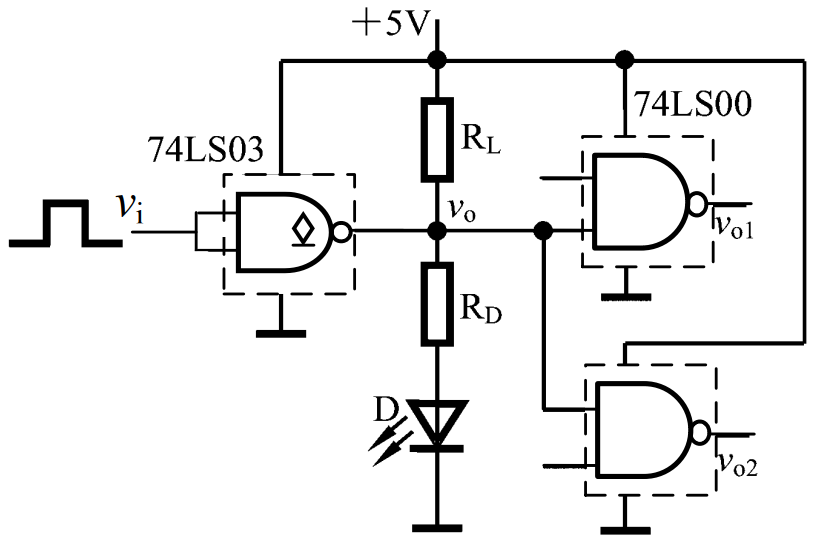
\includegraphics[width=0.5\textwidth]{OC}
	\caption{OC门电路}
\end{figure}
其中,$R_L$的范围有下列等式标定:
$$
R_{\mathrm{Lmax}}=\frac{V_{\mathrm{CC}}-V_{\mathrm{OHmin}}}{nI_{\mathrm{OH}}+m'I_{\mathrm{IH}}},R_{\mathrm{Lmin}}=\frac{V_{\mathrm{CC}}-V_{\mathrm{OLmax}}}{I_{\mathrm{OL}}-mI_{\mathrm{L}}}
$$
\subsection{流水灯电路}
用 D 触发器设计实现模 4 计数器, 用与非门设计实现 2/4 线译码器,主要设计如下图所示:
\begin{figure}[!ht]
	\centering
	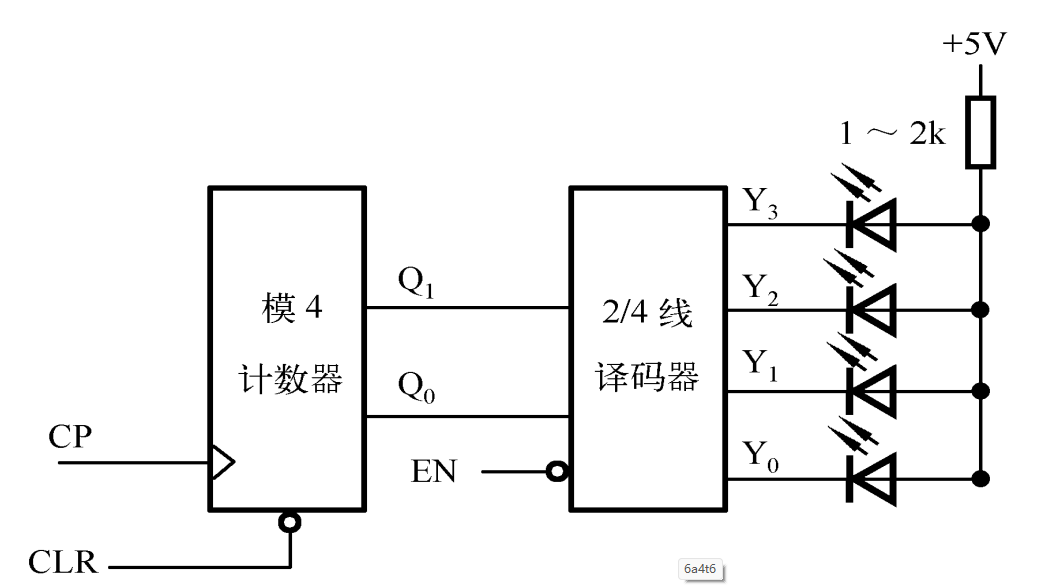
\includegraphics[width=0.7\textwidth]{frame}
	\caption{整体框架}
\end{figure}
\begin{figure}[!ht]
	\centering
	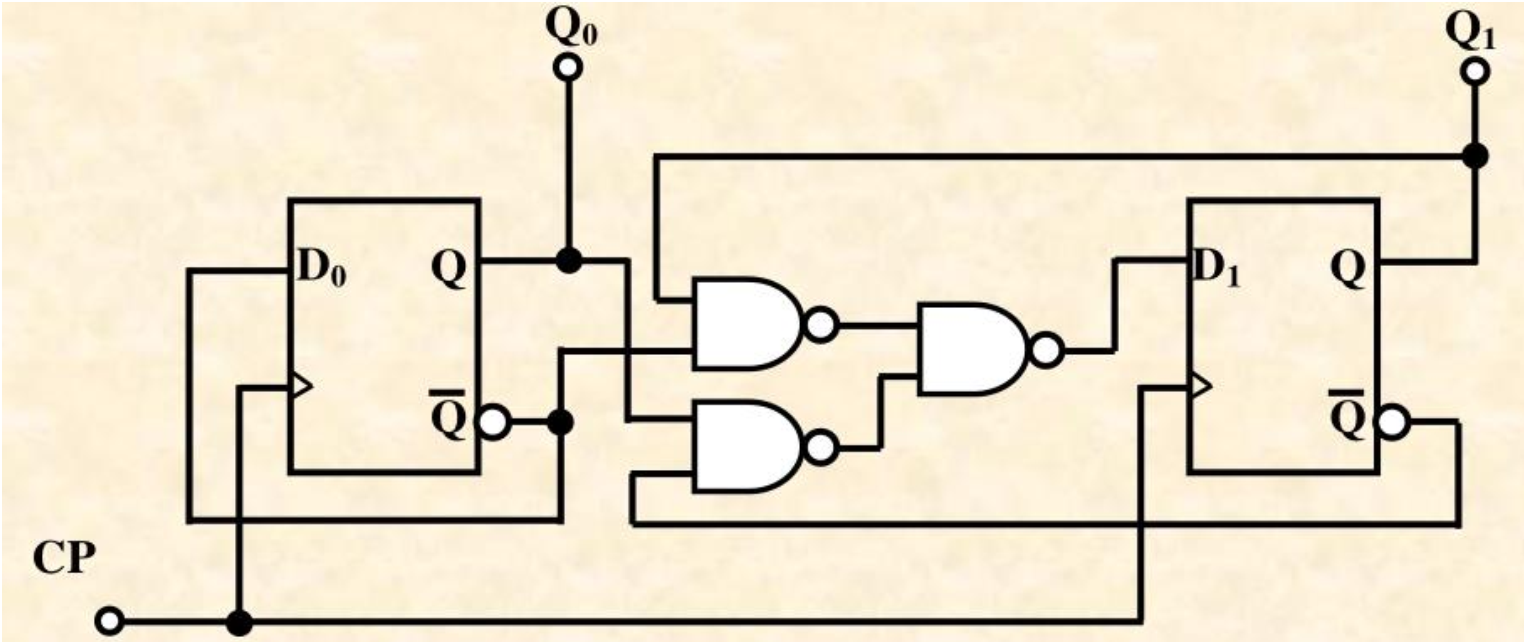
\includegraphics[width=0.7\textwidth]{Cal}
	\caption{模四计数器(用74HC74和74HC00实现)}
\end{figure}
\begin{figure}[!ht]
	\centering
	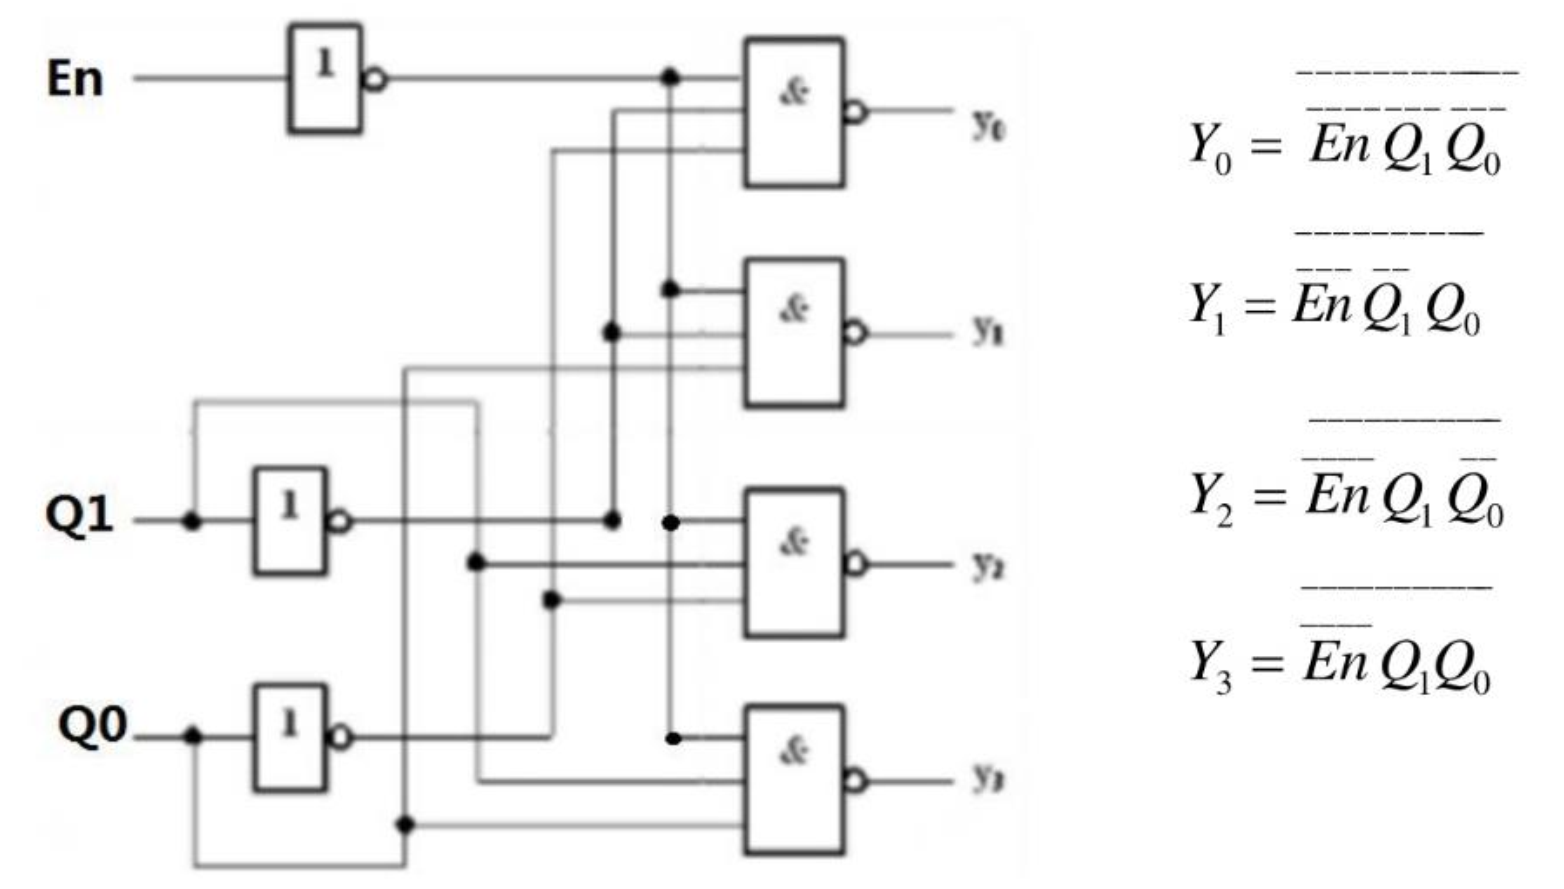
\includegraphics[width=0.7\textwidth]{yimaqi}
	\caption{译码器(用两个74HC10实现)}
\end{figure}
\section{实验内容}
\subsection{OC 门实验}
取发光二极管D正向导通压降$ Vi=1.5V$, 导通电流 2mA, 计算限流电阻$R_o$,负载电阻 $\mathrm{R}_{\mathrm{Lmax}},\quad\mathrm{R}_{\mathrm{Lmin}}$
调整信号源,使其输出 1kHZ、4V 的正方波,将其连接到 $v_i$点,使用示波器“直流耦合”输入方式观察波形,在坐标纸上画出$v_i, v_o, v_{o1}, v_{o2}$的波形,并标出$V_{oH}$,
$V_{oL}$ 的电平值
\end{document}